% Created 2021-01-24 Sun 22:49
% Intended LaTeX compiler: pdflatex
\documentclass[11pt]{article}
\usepackage[utf8]{inputenc}
\usepackage[T1]{fontenc}
\usepackage{graphicx}
\usepackage{grffile}
\usepackage{longtable}
\usepackage{wrapfig}
\usepackage{rotating}
\usepackage[normalem]{ulem}
\usepackage{amsmath}
\usepackage{textcomp}
\usepackage{amssymb}
\usepackage{capt-of}
\usepackage{hyperref}
\usepackage{minted}
\hypersetup{colorlinks=true, linkcolor=black, filecolor=red, urlcolor=blue}
\usepackage[turkish]{babel}
\author{Eren Hatırnaz}
\date{26 Ocak 2020}
\title{Yazılım Gündemi - 2020/04\\\medskip
\large 20-26 Ocak 2020}
\hypersetup{
 pdfauthor={Eren Hatırnaz},
 pdftitle={Yazılım Gündemi - 2020/04},
 pdfkeywords={},
 pdfsubject={},
 pdfcreator={Emacs 27.1 (Org mode 9.3)},
 pdflang={Turkish}}
\begin{document}

\maketitle
\tableofcontents \clearpage\shorthandoff{=}

\begin{center}
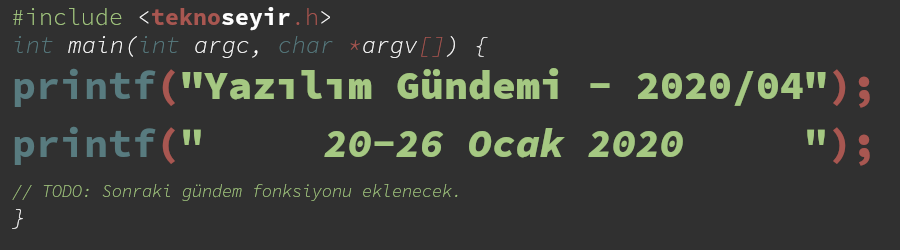
\includegraphics[width=.9\linewidth]{gorseller/yazilim-gundemi-banner.png}
\end{center}

\begin{center}
\href{../03/yazilim-gundemi-2020-03.pdf}{< Önceki Gündem} | \textbf{20-26 Ocak 2020} | \href{../05/yazilim-gundemi-2020-05.pdf}{Sonraki Gündem >}

\href{https://teknoseyir.com/blog/yazilim-gundemi-2020-04}{TeknoSeyir'de Oku}
\end{center}

\section{MEB ve BTG, \href{https://www.meb.gov.tr/1-milyon-meslek-lisesi-ogrencisine-yazilim-egitimi/haber/20138/tr}{"Delphi Eğitimi Protokolü" imzaladılar}}
\label{sec:org464c067}
Milli Eğitim Bakanlığı (MEB) ve \href{https://www.btgrubu.com/}{Bilişim ve Teknoloji Grubu (BTG)} (Delphi dilini
geliştiren Embarcadero firmasının Türkiye Distribütörü) arasında bu hafta
\href{https://www.btgrubu.com/wp-content/uploads/2020/01/MEB-BTG-Protokol-1.pdf}{imzalanan protokole} göre 1 milyon meslek lisesi öğrencisine Delphi programlama
dili öğretilecekmiş. Türkiye yazılım camiasının bu hafta en çok konuştuğu konu
buydu, o yüzden ben de biraz uzun bahsedeceğim bu konudan.

Türkiye yazılım camiasının birçoğu bu haberi HackerNews'de paylaşılan \href{https://jonlennartaasenden.wordpress.com/2020/01/20/turkey-buys-delphi-licenses-for-an-estimated-one-million-students/}{bu blog
yazısı} ile öğrendi. Şimdi başlık düzeltilmiş durumda fakat başlığın ilk hali
şöyleydi: Turkey buys Delphi licenses for an estimated one million student
[bunu yazının bağlantısındaki ilgili kısımdan siz de teyit edebilirsiniz].
Başlıkta "buys" (satın almak) kelimesinin geçmesinden dolayı herkes bu haberi
"MEB, 1 milyon öğrenci için Delphi lisansı satın aldı" olarak algıladı. \href{https://www.timeturk.com/meb-den-1-milyon-meslek-lisesi-ogrencisine-yazilim-egitimi/haber-1337091}{Türkçe
kaynaklarda} herhangi bir satın almadan ya da ücretten bahsedilmiyor fakat yine
de başlığın yanlış yazılmasından dolayı çoğumuz da yanlış anladık. Ben de
TeknoSeyir Sosyal'de paylaştığım gönderide "satın aldı" olarak yazmıştım fakat
gün içerisinde herhangi bir satın almanın olmadığını öğrendiğimizde benimle
birlikte yanlış anlayan çoğu kişi ilgili düzeltmeleri yaptılar. Daha sonra
yayınlanan protokol metininde de şu maddenin olması içimize biraz olsun su
serpti:

\begin{quote}
Madde 11- BTG düzenlenen faaliyetlerde öğrenci ve öğretmenlerden hiçbir ad
altında ücret alamaz.
\end{quote}
[Gerçi bu maddede "öğrenci ve öğretmenlerden ücret alınamaz" deniyor ama yine
de protokolün devamındaki metinlerde MEB tarafı için de herhangi bir ödeme
gözükmüyor.]

Yukarıdaki yanlış anlamadan dolayı çoğumuzun ilk argümanı "Delphi gibi eski ve
günümüzde kullanılmayan bir dil için bu kadar kamu kaynağının aktarılması
saçmalıktır" oldu. Aslında bakarsanız yanlış anlaşılma giderildikten sonra da
argümanımızda çok fazla bir değişiklik olmadı. Sonuç olarak kamu kaynaklarından
tek bir kuruş ödeme yapılmamış olsa bile Delphi gibi eski, sektörde neredeyse
hiç kullanılmayan, kapalı kaynak, ücretli ve topluluk desteği olmayan bir
programlama dilinin 2020 yılında gençlere öğretilmek istenmesi kabul edilemez.
Sosyalde çeşitli gönderiler altında argümanlarımızı yazmıştım onları bütünlüklü
bir hale getirmek gerekirse:

\begin{itemize}
\item Delphi kapalı kaynak, ücretli ve tek firmanın elinde olan bir programlama
dilidir. Her ne kadar gençler bu programlama dili ve araçlarına okullarında
kurulu olan laboratuvardan ücretsiz olarak erişilebilir olsa da bu işin bir
de mezuniyet sonrası var. Delphi dilini ve araçlarını ticari olarak
kullanmak isterseniz yıllık 1700€ ücret vermeniz gerekiyor. Delphi Community
Edition isimli bir sürümü de mevcut fakat onun için de yıllık kazancınızın
5.000\$ altında olması gerekiyor, bu miktarı geçerseniz ücret lisans almanız
gerekiyor. Açık kaynak ve özgür lisanslı, ücretsiz programlama dilleri ile
geliştirme yapıp tek kuruş lisans ücreti ödememek varken niye Delphi
kullansın bu gençler?
\item Çeşitli platformlardaki tartışmalarda karşıma çıkan argümanlardan birisi de
"Delphi öğrenmesi kolay, sürükle\&bırak mantığıyla uygulama tasarlayıp,
derleyip, çalıştırabileceğiniz bir dil. Hem hızlı uygulama çıkarabilmek hem
de görsellikten dolayı eğitim için uygundur". Bu argümanın katıldığım
noktaları var. Özellikle o yaşlardaki gençlerin daha çok sonuç odaklı olarak
yazdıkları kodların çıktılarını hemen görmek istemelerini gayet anlayışla
karşılayabiliyorum ve Delphi geliştirme ortamının bunu sağlayabildiğini
biliyorum. Benim çekincem daha çevremde gözlemlediğim bazı durumlardan
kaynaklanıyor. Şöyle ki: Meslek yüksekokulunda okurken, meslek lisesinden
gelen arkadaşların Microsoft Frontpage ve Adobe Dreamvewer gibi
sürükle\&bırak modeli üzerine kurulu uygulamalarda HTML ve CSS
öğrendiklerinden dolayı, üniversitede zorluklar yaşadılar. Çoğu HTML ve CSS
kodlarını görmemişti. Üniversitedeki hocamız da doğal olarak sürükle\&bırak
yerine kod yazarak ders işlediğinden dolayı bu arkadaşların derslerden geri
kaldıklarını gözlemledim. Elbette bu örnekler ile Delphi'yi kıyaslamak çok
doğru olmayacaktır ama günümüzde pek kullanılmayan bir geliştirme ortamı
olması dolayısıyla gençlerin günümüz yazılım geliştirme süreçlerine entegre
olmalarını zorlaştıracağını düşünüyorum.
\item Karşılaştığım argümanlardan bir diğerine gelecek olursak: "Delphi
kullanarak, sürükle\&bırak modelinde geliştirdiğiniz uygulamaları çok kolay
şekilde platformlar-arası (cross-platform) uygulama haline getirebilirsiniz.
Yazdığınız uygulamaları Windows, macOS, GNU/Linux ve Android gibi
sistemlerde çalıştırabilirsiniz. Bunu yapabilecek başka bir platform
öneriniz var mı?". Bu argümana cevabım ise Delphi IDE'sinin üzerine kurulu
olduğu sürükle\&bırak geliştirme modelinin günümüz geliştirme süreçlerinde
pek de aranan bir şey olmadığı, dolayısıyla da önerimin olmadığı yönünde
oldu. Her ne kadar Delphi gibi sürükle\&bırak modeliyle olmasa da bugün
platformlar-arası uygulama geliştirmeye yarayan birçok framework mevcut.
ElectronJS, Qt, Flutter vb. sistemleri örnek olarak sayabiliriz. Günümüzdeki
bazı geliştirme modelleri, özellikle de ElectronJS'in üzerine kurulu olduğu
model, benim de hoşuma gitmemesine rağmen sektör tarafından son derece kabul
edilmiş ve yaygın uygulama geliştirme modelleri olarak karşımızdalar.
\end{itemize}

Benim argümanların genel olarak bu şekildeydi. Özetleyecek olursam: Delphi dili
ve araçlarıyla kişisel olarak bir problemim yok ama maalesef bu dil ve araçlar
günümüz için geçerli seçenekler değil. Gençlere açık kaynak ve özgür lisanslı,
ücretsiz, topluluk tarafından desteklenen ve geliştirilen diller öğretmemizin
daha doğru olacağını düşünüyorum. Nitekim Bilgisayar Mühendisleri Odası da
hemen hemen bu yazdıklarıma yakın bir şekilde \href{https://www.bmo.org.tr/2020/01/23/mebin-teknik-liselerde-yazilim-egitimi-yontemi-cagdisidir/}{kendi bildirilerini yayınladılar}
ve Milli Eğitim Bakanlığı'ndan bu protokolü iptal etmelerini talep ettiler.

Bu konuda siz ne düşünüyorsunuz? Yorumlar bölümünde konuşalım.
\section{JetBrains, IntelliJ tabanlı IDE'leri için \href{https://blog.jetbrains.com/idea/2020/01/intellij-based-ide-features-roadmap-for-2020/}{2020 yeni özellikler yol haritası}nı yayınladı}
\label{sec:org07920a7}
Geçtiğimiz senedeki yazılım gündemlerinin birinde (bkz: \href{../../2019/22/yazilim-gundemi-22.pdf}{Yazılım Gündemi - 22})
JetBrains'in, IntelliJ Platformu için yayınladığı 2020 yol haritasını
konuşmuştuk. O yazıda daha çok platformun daha derinlerindeki özellikler ile
ilgili yol haritasından bahsetmişlerdi. Bu hafta yayınladıkları "IntelliJ-based
IDE Features Roadmap for 2020" başlıklı yazı ile daha çok biz geliştiricilerin
etkileştikleri yerlere ilgili özelliklerin yol haritasını yayınladılar. Şöyle
birkaç alt başlığa göz atalım:

\subsection{IDE'yi genel amaçlı metin düzenleyici olarak kullanabilme}
\label{sec:org5cb234e}
\begin{center}
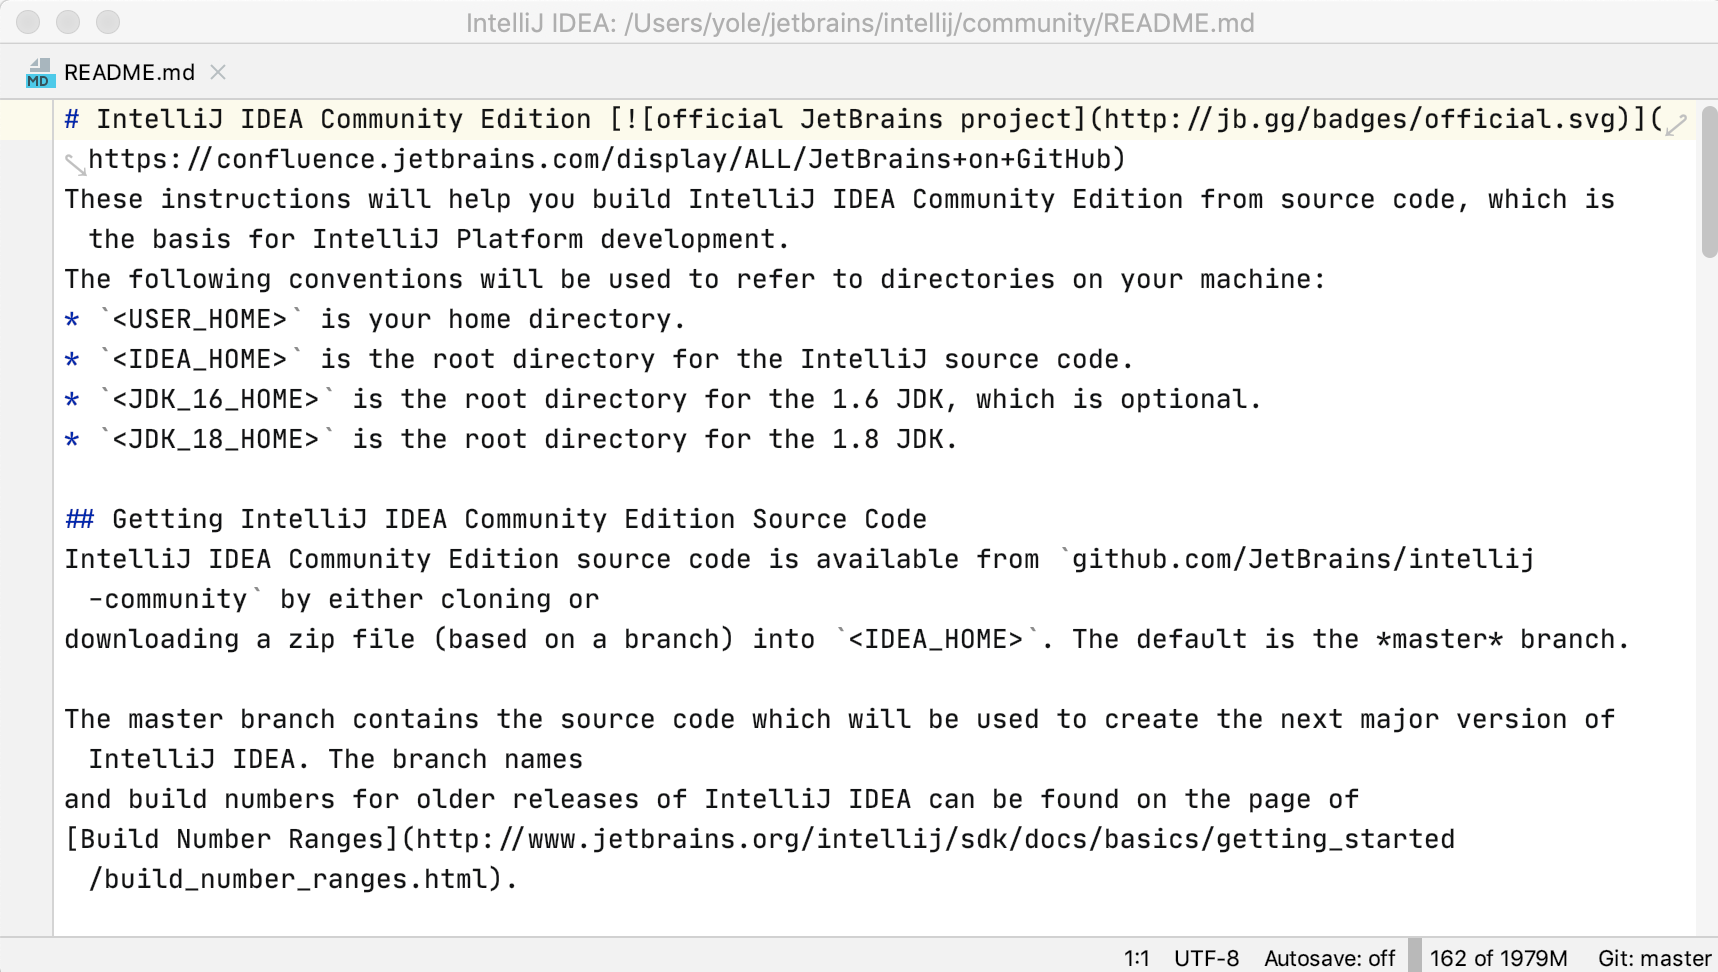
\includegraphics[width=.9\linewidth]{gorseller/jetbrains-text-mode.png}
\end{center}

JetBrains IDE'lerinin kullanıcıları üzerlerinde çalıştıkları projelere ek
olarak aynı zamanda çeşitli farklı dosyaları da bu IDE'ler ile düzenlemek
istiyorlarmış. Mesela log dosyalarını görüntülemek, sunucu ayar dosyalarını
düzenlemek gibi. Elbette bunu yapmak mümkün fakat JetBrains IDE'leri daha çok
proje tabanlı çalışmaya uygun oldukları için tek bir dosya açsalar bile sanki
bir proje açmışlar gibi gözüküyordu ve bazı yavaşlamalar oluyordu. 2020
yılında artık JetBrains takımı, IDE'lerini genel amaçlı metin düzenleme (text
editor) işleri için de kolayca kullanılabilir hale getirmeyi planlıyorlar.
Bunun için de özel bir mod hazırlıyorlarmış. Benim tahminim büyük ihtimal
komut satırından bir dosyayı açarken "phpstorm --text-mode deneme.log" gibi
bir komut çalıştıracaksınız ve bu mod o şekilde açılacak. Elbette bu modun
daha hızlı açılabilmesi için çoğu IDE özellikleri çalışmayacak fakat
kullanıcıların birçoğunun ihtiyaçlarını karşılayacaktır. Aynı zamanda bu
moddan normal IDE moduna geçmek için de yol olacak deniyor.
\subsection{Makine öğrenmesi tabanlı kod tamamlama önerileri}
\label{sec:org19d4c4b}
JetBrains IDE'lerinin en meşhur özelliklerinden biri de çok gelişmiş kod
tamamlama ve öneri sisteminin olmasıdır. Benim de kullandığım zamanlarda
gerçekten çok işime yarayan özelliklerden biriydi. Biraz da kavramın
popülerleşmesinden dolayı olsa gerek artık bu öneri sistemine "makine
öğrenmesi" ekleyeceklermiş. IDE'lerin son sürümlerinde bazı makine öğrenmesi
yöntemlerinden faydalanmışlar ama sonraki sürümlerinde bu daha da
geliştireceklerini ve geliştirme sürecinin çok büyük bir eforunu bu kısım
üzerine yoğunlaştırdıklarını belirtmişler.
\subsection{Geliştirme ortamının kurulması}
\label{sec:org09390cc}
JetBrains takımı artık IDE'leri kuranlara yardımcı olmak için geliştirme
ortamıyla ilgili bazı kurulumlarda da yardımcı olacakmış. Mesela Git'in
kurulması ya da bir JDK sürümünün kurulması gibi. Böylece JetBrains
IDE'lerini kullananlar geliştirme ortamlarını daha hızlı bir şekilde hazır
hale getirebilecekler. Şahsen ben bu tarz kurulumları yine kendim elle yapmak
isterim ama istemeyen geliştiriciler için güzel bir kolaylık olacaktır diye
düşünüyorum.

Bu özelliklerden bazılarını IDE'lerinin 2020.1 sürümlerinde kullanıma
açılacağını belirtmişler. Nitekim yine bu hafta \href{https://blog.jetbrains.com/idea/2020/01/intellij-idea-2020-1-eap/}{yayınlanan IntelliJ IDEA
2020.1}'de bu sözleri yerine getiriyorlar. Henüz erken erişim programında olan
bu sürüm ile birlikte yukarıda "Geliştirme ortamının kurulması" alt başlığında
bahsettiğim JDK sürümleri indirme özelliğini eklemişler.

\url{gorseller/jetbrains-jdk-indirme.gif}


2020 yılı yeni özellikler yol haritasının tüm alt başlıkları için konu
başlığına eklediğim bağlantıya; IntelliJ IDEA 2020.1 EAP sürümünün
detaylarıyla ilgili bilgiler için de \href{https://blog.jetbrains.com/idea/2020/01/intellij-idea-2020-1-eap/}{bu bağlantıya} tıklayabilirsiniz.
\section{Microsoft Edge tarayıcısının geliştirici özelliklerine \href{https://blogs.windows.com/msedgedev/2020/01/23/debug-z-index-3d-view-edge-devtools/}{3-boyutlu görüntüleme ekledi}}
\label{sec:org3fed82f}
Geçtiğimiz haftalarda tüm kullanıcılar için Beta programından çıkan
Microsoft'un yeni Chromium tabanlı tarayıcısı Edge'in içerisindeki geliştirici
araçlarına güzel bir özellik eklenmiş. Artık bir web sitesi üzerindeki
elemanları 3 boyutlu olarak inceleyip, özelliklerine bakabileceğiz. Henüz
sadece deneysel (experimental) olan bu özelliği aktifleştirmek için Edge'deki
\textbf{DevTools} kısmını açtıktan sonra \textbf{Settings} sekmesi altından "\textbf{Enable 3D
View}" seçeneğini işaretlemek gerekiyor.

Özelliği daha iyi anlayabilmek adına Twitter'daki Microsoft Edge DevTools
isimli hesabın \href{https://twitter.com/EdgeDevTools/status/1220399837956333569}{paylaştığı videoyu izleyebilirsiniz}.
\section{MySQL 5.6'nın 1 yıllık \href{https://lefred.be/content/mysql-5-6-eol-is-february-2021/}{ömrü kalmış}}
\label{sec:org0c5779d}
\begin{center}
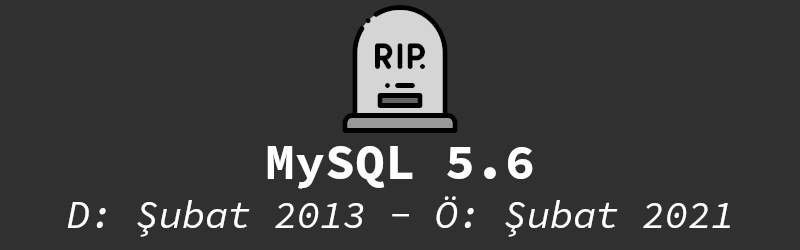
\includegraphics[width=.9\linewidth]{gorseller/mysql56-olum.png}
\end{center}

Bu haber doğrudan biz geliştiricileri ilgilendirmiyor ama dolaylı yoldan da
olsa bizi etkileyebileceği için gündeme almak istedim. MySQL veritabanının 5.6
sürümü Şubat 2021 tarihinde aramızdan ayrılacakmış. Sistem yöneticilerinizi
konuyla ilgili bilgilendirebilirsiniz.
\section{Yaklaşan Etkinlikler}
\label{sec:org3454d88}
\begin{longtable}{|p{8cm}|l|l|}
\hline
Etkinlik İsmi & Yeri & Tarihi\\
\hline
\endfirsthead
\multicolumn{3}{l}{Önceki sayfadan devam ediyor} \\
\hline

Etkinlik İsmi & Yeri & Tarihi \\

\hline
\endhead
\hline\multicolumn{3}{r}{Devamı sonraki sayfada} \\
\endfoot
\endlastfoot
\hline
\href{https://www.meetup.com/Google-Cloud-Developer-Community-Ankara/events/268138124/}{ML in the cloud: Cloud AI Platform} & Ankara & 29 Ocak 19:00\\
\href{https://www.meetup.com/GDGIstanbul/events/268082538/}{CoffeeDroid 5 - Kaldığımız yerden devam edelim} & İstanbul & 29 Ocak 19:00\\
\href{https://www.meetup.com/TeknasyonLabs/events/268053933/}{Geliştirici Savaşları Bölüm 1: Gizli Tehlike} & İstanbul & 30 Ocak 16:00\\
\href{https://www.meetup.com/Facebook-Developer-Circle-Ankara/events/268055524/}{An Inside Look: Indie Games Accelerator} & Ankara & 30 Ocak 18:30\\
\href{https://www.meetup.com/IBMCloudTR/events/268163839/}{OpenShift ile DevOps Pratiklerini Nasıl Deneyimleriz?} & İstanbul & 30 Ocak 19:00\\
\href{https://www.meetup.com/Coffee-And-React-Native-\%25C4\%25B0stanbul/events/vzxzkrybcdbcb/}{Coffee and React Native} & İstanbul & 1 Şubat 11:00\\
\href{https://kommunity.com/flutter-turkiye/events/istanbul-coffee-and-talk}{Istanbul Coffee and Talk - 1 (Flutter Turkiye)} & İstanbul & 2 Şubat 13:00\\
\href{https://www.meetup.com/GDG-Cloud-Izmir/events/268107353/}{Serverless Application with Flutter and Cloud Functions} & İzmir & 2 Şubat 13:00\\
\href{https://kommunity.com/cloud-and-serverless-turkey/events/istegelsin-serverless-aws-lambda-mimarisi-ve-production-tecrubeleri}{İstegelsin Serverless AWS Lambda Mimarisi ve Production Tecrübeleri} & İstanbul & 4 Şubat 18:30\\
\href{https://kommunity.com/cloud-and-serverless-turkey/events/aws-fundamentals-computer-networking-security-storage-and-more-ankara}{AWS Fundamentals: Computer, Networking, Security, Storage and more} & Ankara & 5 Şubat 18:30\\
\href{https://kommunity.com/reactjs-istanbul/events/tanisma-toplantisi-first-meeting}{Tanışma toplantısı! (ReactJS Istanbul)} & İstanbul & 5 Şubat 19:00\\
\href{https://kommunity.com/indiehackers-istanbul-meetup/events/lets-meet-and-catch-a-little-up}{Indie Hackers Istanbul Meetup} & İstanbul & 8 Şubat 17:00\\
\hline
\end{longtable}
\section{Diğer Haberler}
\label{sec:org5bc14ce}
\begin{itemize}
\item Microsoft, yeni Node tabanlı tarayıcı otomasyonu \href{https://css-tricks.com/playwright/}{projesini yayınladı}:
\href{https://github.com/microsoft/playwright}{Playwright}.
\item ProtonVPN tüm uygulamalarını \href{https://protonvpn.com/blog/open-source/}{açık kaynak hale getirdi}.
\item Android Studio 4.0 Canary 9 \href{https://androidstudio.googleblog.com/2020/01/android-studio-40-canary-9-available.html}{sürümü yayınlandı}.
\item Birçok AndroidX kütüphanesine \href{https://developer.android.com/jetpack/androidx/versions/all-channel\#january\_22\_2020}{güncelleme geldi}.
\item Google Cloud ailesinin \href{https://cloud.google.com/blog/products/identity-security/introducing-google-clouds-secret-manager}{yeni üyesi tanıtıldı}: \href{https://cloud.google.com/secret-manager/docs}{Secret Manager}.
\item Intel tarafından geliştirilen Ray Tracing motorunun 2.0.0 \href{https://github.com/ospray/ospray/releases/tag/v2.0.0}{sürümü yayınlandı}.
\item Pharo programlama dilinin 8.0 \href{http://pharo.org/news/pharo8.0-released}{sürümü yayınlandı}.
\item Seq programlama dilinin v0.9.3 \href{https://github.com/seq-lang/seq/releases/tag/v0.9.3}{sürümü yayınlandı}.
\item Flamegraph kütüphanesinin v0.2.0 \href{https://github.com/flamegraph-rs/flamegraph/releases/tag/v0.2.0}{sürümü yayınlandı}.
\end{itemize}
\section{Lisans}
\label{sec:orge994b68}
\begin{center}
\begin{center}

\includegraphics[height=1.5cm]{../../../img/CC_BY-NC-SA_4.0.png}
\end{center}

\href{yazilim-gundemi-2020-04.pdf}{Yazılım Gündemi - 2020/04} yazısı \href{https://erenhatirnaz.github.io}{Eren Hatırnaz} tarafından \href{http://creativecommons.org/licenses/by-nc-sa/4.0/}{Creative Commons
Atıf-GayriTicari-AynıLisanslaPaylaş 4.0 Uluslararası Lisansı} (CC BY-NC-SA 4.0)
ile lisanslanmıştır.
\end{center}
\end{document}
